\section*{\begin{tabular*}{\linewidth}{@{}l @{\extracolsep{\fill}} r@{}}
Nr.~1 & MLB~85/1-3-1 \\
\end{tabular*} 
}

\textsf{\textbf{Maluba (Lua; Fpl.~230)}}

\vspace{1em}

\noindent\begin{tabular}{@{}rl@{}}
\textbf{Feldarbeit:} & \begin{tabular}[t]{@{}l@{}}\textbf{05.09.--08.09.1985}\\ \textbf{(M. K. H. Eggert/F. Nikulka)}\end{tabular} \\ 
\textbf{Abb.:} & \textbf{\ref{fig:MLB85_1_Zeichnung}--\ref{fig:MLB85_1_14C-Kalibration}} \\
\textbf{Tab.:} & \textbf{\ref{tab:MLB85-1-3-1_Funde}--\ref{tab:MLB85_1-3-1_14C-Daten}}\\
\textbf{Taf.:} & \textbf{25.1--26.8} \\ 
\textbf{Lit.:} & \textbf{\textsc{Eggert}~1987b} \\ 
\end{tabular}

\begin{figure*}[p]
 \centering
 \includegraphics[width=.9\textwidth]{fig/MLB85-1.pdf}
 \caption{MLB 85/1: Planum bei etwa 0,4 m unter der rezente Oberfläche und Profil der Süd-Nord-orientierten Uferböschung.}
 \label{fig:MLB85_1_Zeichnung}
\end{figure*}

\begin{figure*}[p]
\centering
 \begin{subfigure}{\columnwidth}
 \centering
 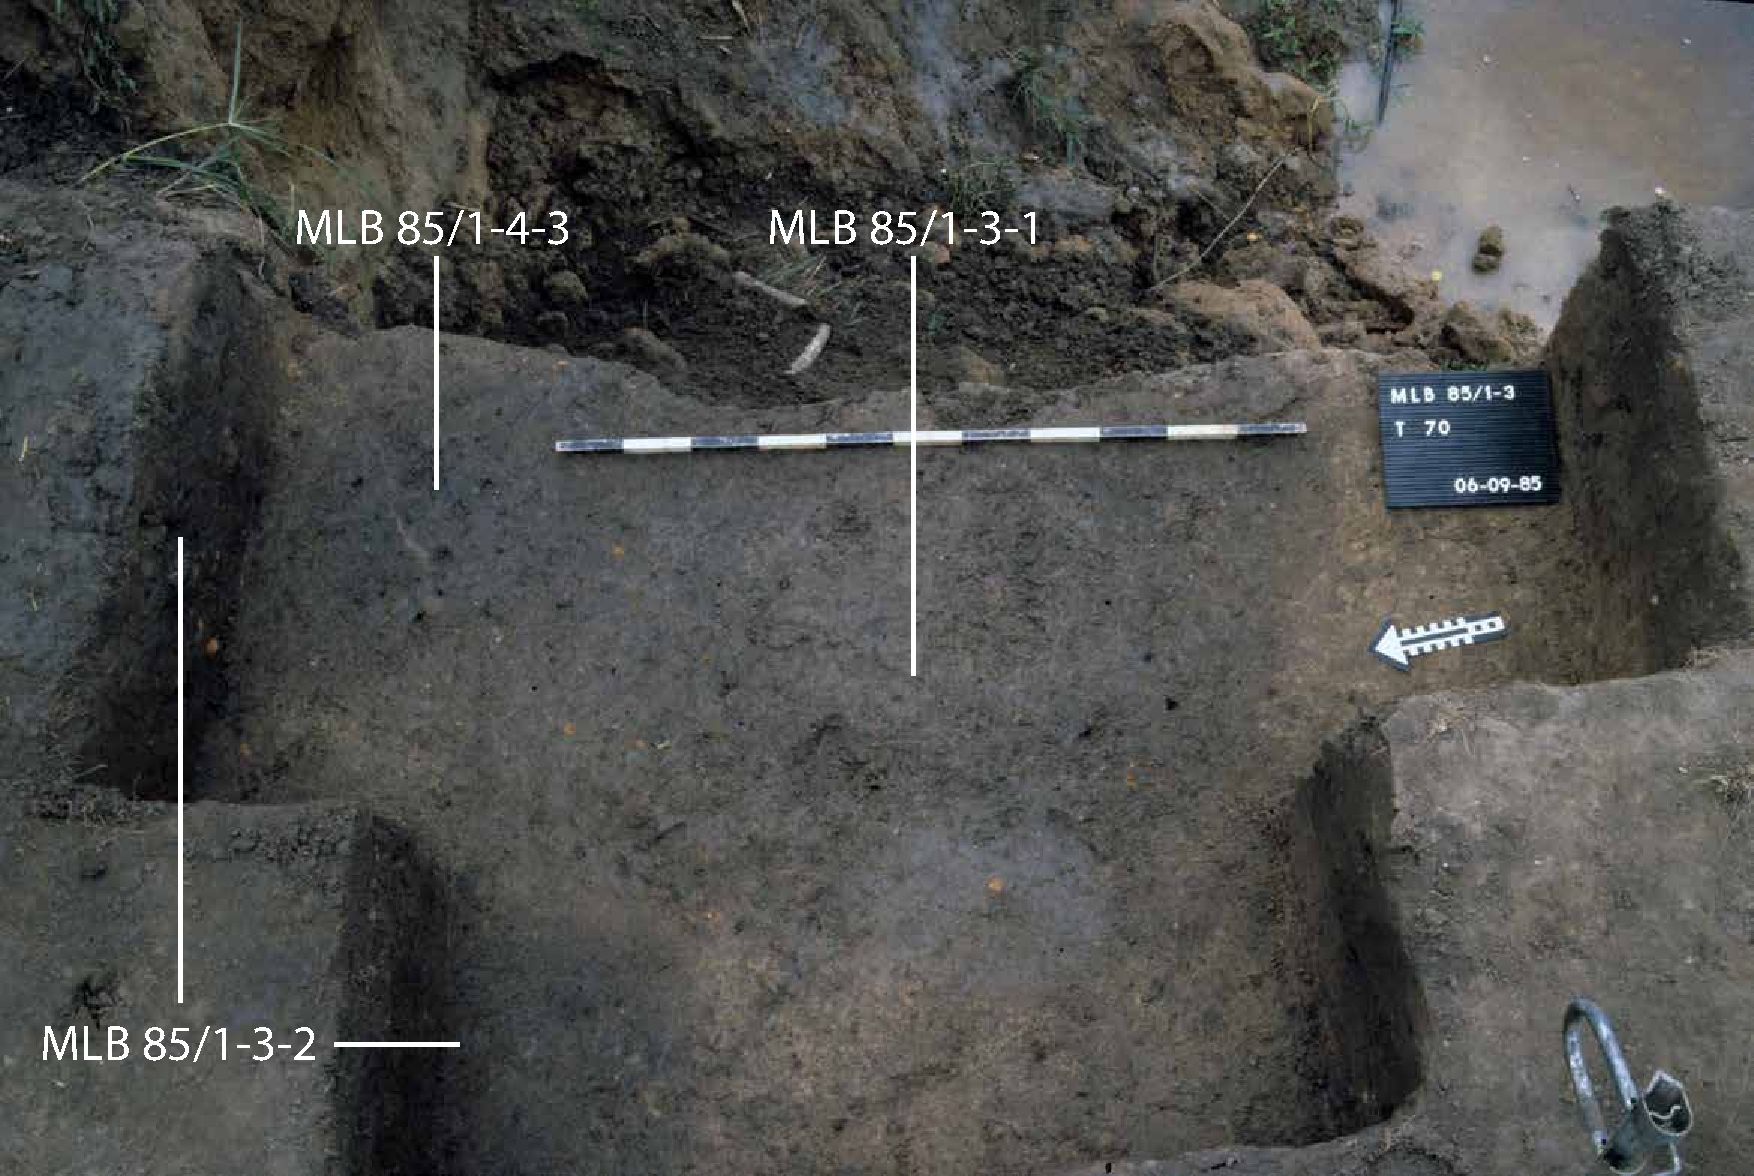
\includegraphics[width=\columnwidth]{fig/MLB85-1-3_T70_E85-031-1_kompr.pdf}
 \caption{Planum 3 (0,45\,m u.~Obfl.)}
 \label{fig:MLB85_1_PlanaT70}
 \end{subfigure}\hfill
 \begin{subfigure}{\columnwidth}
 \centering
 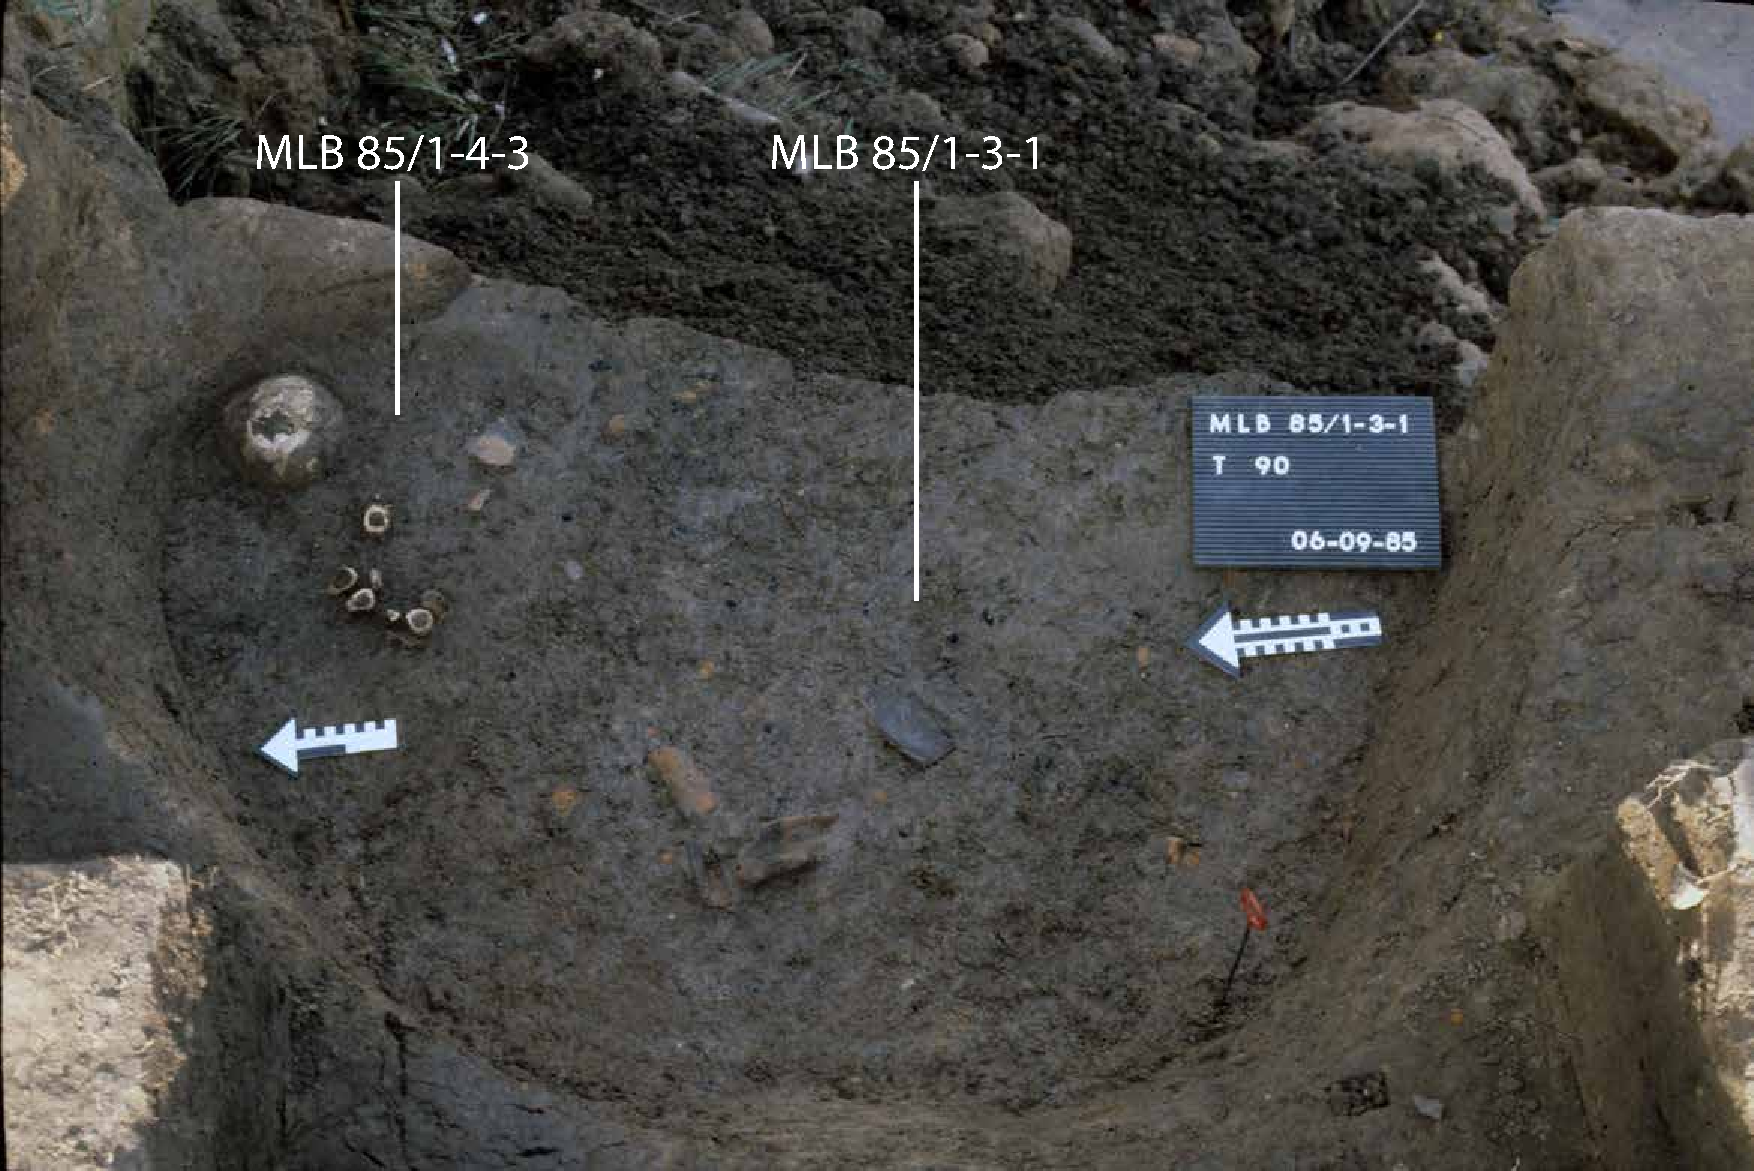
\includegraphics[width=\columnwidth]{fig/MLB85-1-3-1_T90_E85-031-15_kompr.pdf}
 \caption{Planum 4 (0,60\,m u.~Obfl.)}
 \label{fig:MLB85_1_PlanaT90}
\end{subfigure}
 \caption{MLB 85/1: Planum 3 und 4 (Fotos: M. K. H. Eggert, 1985).}
 \label{fig:MLB85_1_PlanaT70+90_Foto}
\end{figure*}

\begin{table*}[p]
	\centering
	%	%\begin{minipage}{.66\textwidth}
	{\footnotesize \begin{sftabular}{@{}lrrrr@{}}
\toprule
   \textbf{Fundkategorie} &  \textbf{Anzahl} &    \textbf{\%} &  \textbf{Gewicht (kg)} &    \textbf{\%} \\
\midrule
 gebrannter Lehm &       1 &   0,3 &          0,10 &   2,0 \\
         Keramik &     305 &  99,0 &          4,49 &  95,7 \\
           Stein &       2 &   0,6 &          0,11 &   2,3 \\
\bottomrule
\end{sftabular}}
	\caption{MLB~85/1-3-1: Anteil verschiedener Fundmaterialien.}
	\label{tab:MLB85-1-3-1_Funde}
	%	%\end{minipage}
\end{table*}

% MLB 85/102 == MLB 85/1-3-1
\paragraph{Grabung und Befunde}\hspace{-.5em}|\hspace{.5em}%
Die Prospektionen in Maluba erbrachten eine Reihe von Gruben. Ausgrabungen an zwei getrennten Stellen innerhalb des Dorfes fanden im Anschluss an die Prospektion des Lua statt. Im etwa 3--4\,m hohen, tonigen Uferprofil des Lua wurden die Reste von vier teilweise freierodierten, tiefen Gruben untersucht: zwei Gruben mit Keramik der Batalimo-Maluba-Gruppe (Kat.-Nr.~1--2) sowie zwei weitere mit (sub)rezentem Fundmaterial (Kat.-Nr.~4--5).\footnote{Nach schweren Regenfällen stürzte die Grabung MLB~85/2 (Kat.-Nr.~4) teilweise ein. Im Anschluss wurde ausschließlich die Grabung MLB~85/1, in welcher die beiden Gruben MLB~85/1-3-1 (Kat.-Nr.~1) und MLB~85/1-3-2 (Kat.-Nr.~2) erfasst wurden, fortgeführt. Die Grabung MLB~85/1 erfasste auch die jüngere Sekundärbestattung MLB~85/1-4-3 (Kat.-Nr.~3). An mehreren Stellen im Dorf wurden an der Oberfläche sichtbare Skelettreste beobachtet. Diese waren den Einwohnern auf Nachfrage hin bekannt.} Im Zuge der ursprünglichen Prospektion in Maluba wurde die spätere Grabungsstelle MLB~85/1 als Survey-Komplex MLB~85/102 aufgenommen.\footnote{Im Verlauf der Bearbeitung zeigte sich, dass die Funde aus dem Survey-Komplex MLB~85/102 Teil der Grube MLB~85/1-3-1 sind. Während der Grabung in Schnitt MLB~85/1 wurde eine weitere Grube zuerst angeschnitten und später unter der Bezeichnung MLB~85/1-3-2 (Kat.-Nr.~2) ebenfalls ausgegraben.} Der Befund war durch einen Erdrutsch freigelegt worden und die Abbruchkante des Uferprofils war zum Zeitpunkt der Grabung etwa 3\,m vom eigentlichen Ufer entfernt und lag mehr als 4,5\,m über dem Wasserspiegel.

Die unter der Kennung MLB~85/1-3-1 ausgegrabene Grube ist kesselförmig und war bis etwa 1,1\,m unter die rezente Oberfläche erhalten (Abb.~\ref{fig:MLB85_1_Zeichnung}). Sie hat einen Durchmesser von zirka 1,5\,m, die Wandungen sind vertikal bis steilschräg überkippt und die Sohle konvex bis wellig mit fließenden Ecken. Die Befundgrenzen sind verwaschen bis fließend und waren aufgrund von Bioturbation schwer zu erfassen. Die ursprüngliche Oberfläche lässt sich nicht mehr rekonstruieren. Im oberen Bereich des erhaltenen Profils ist eine zirka 0,3\,m mächtige dunkle Lage erkennbar (Abb.~\ref{fig:MLB85_1_Zeichnung}: Schicht~1), deren Farbe sich nicht von jener der Grubenfüllung unterscheidet. In dieser Schicht fand sich fast 1/3 der insgesamt aus dem Befund vorliegenden Batalimo-Maluba-Keramik sowie Vertreter anderer Stilgruppen (Abb.~\ref{fig:MLB85-1_KeramikStilgruppen}). Dies legt den Schluss nahe, dass es sich um einen in späterer Zeit aufgearbeiteten Teil der Grube handelt.

An der Unterkante des zweiten Abtrages, bei etwa 0,35\,m unter der rezenten Oberfläche, wurde eine Lage hellen, lehmigen Sediments erfasst. Die eigentlichen Konturen der Grube zeichneten sich erst im dritten Abtrag deutlich ab (Abb.~\ref{fig:MLB85_1_Zeichnung}).\footnote{Ab dieser Tiefe wurden die Abträge nicht mehr bis zu den Grenzen des Grabungsschnittes abgetieft. Nur die eigentliche Verfüllung der Grube in vier weiteren, künstlichen Abträgen ausgegraben.} Im nördlichen Profil des Grabungsschnitts und im westlichen Teil des dritten Planums wurde eine weitere Grube erfasst, die ebenfalls Keramik der Batalimo-Maluba-Gruppe enthielt (MLB~85/1-3-2; Kat.-Nr.~2). Nahe der nordwestlichen Ecke des Schnittes, kurz vor dem Profil, wurden im vierten Abtrag (0,45--0,60\,m u.~Obfl.) ein Schädel und mehrere Langknochen gefunden (Abb.~\ref{fig:MLB85_1_PlanaT70+90_Foto}).\footnote{Der entsprechende Befund wurde unter der Kennung MLB~85/1-4-3 ausgegraben (Kat.-Nr.~3).} Ab dem fünften Abtrag zeichnete sich um die Knochen herum eine deutliche runde Verfärbung ab. Die angelegten Profile ergaben weder eine stratigraphische Relation zwischen den beiden Gruben MLB~85/1-3-1 und MLB~85/1-3-2, noch zwischen der Grube MLB~85/1-3-1 und der Sekundärbestattung MLB~85/1-4-3.\footnote{Es konnte aber festgestellt werden, dass die Sekundärbestattung MLB~85/1-4-3 (Kat.-Nr.~3) in die Verfüllung der Grube MLB~85/1-3-2 (Kat.-Nr.~2) eingreift. Siehe Abb.~\ref{fig:MLB85_1_Zeichnung}: oben, A--B und E--F; \ref{fig:MLB85-143}).}

\vspace{.5em}\noindent Die Grabung erbrachte den folgenden stratigrafischen Befund (Abb.~\ref{fig:MLB85_1_Zeichnung}):
\begin{itemize}[leftmargin=*, labelindent=1.5em, noitemsep, topsep=0pt]
\item [(1)] Deckschicht, 10YR 3/2 bis 3/3, stark humoser, lehmiger Sand
\item [(2)] Grubenverfüllung, 10YR 3/2, stark holzkohlehaltig, humos, lehmiger Sand
\item [(2a)] Angeschnittene Grube MLB~85/1-3-2 (Kat.-Nr.~2), wie (2), 10YR 3/2, lehmiger Sand
\item [(3)] Grubensohle, 10YR 4/3 bis 3/3, fundarm, sandiger Lehm
\item [(4)] Anstehendes, 10YR 5/6, sandiger Lehm
\item [(4a)] Wie (4), 10 YR 5/6 bis 4/3, sandiger Lehm
\item [(5)] Dunkle Linsen aus sandigem Lehm, 10YR 4/3 bis 3/3
\end{itemize}

\begin{figure*}[tb]
	\centering
	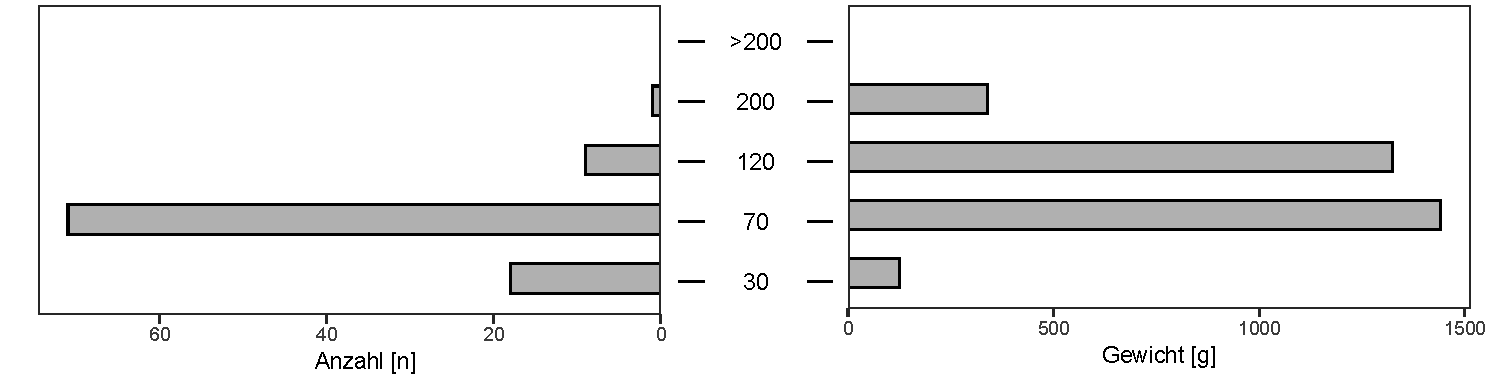
\includegraphics[width=\textwidth]{fig/9-1_MLB85-131_Fragmentierung_2.pdf}
	\caption{MLB~85/1-3-1: Fragmentierungsgrad der Scherben (n~=~99; Größenklassen siehe Anm.~\ref{ftn:Keramik_Fragmentierung}).}
	\label{fig:Fragmenierung_MLB85-131}
\end{figure*}

\columnbreak\paragraph{Keramik\vspace{.5em}}\mbox{}\\
\begin{tabular}{@{}lrl@{}}
Ausgesondert: & 1234\,g & \\
Bearbeitet: & 3228\,g & (72\,\%) \\
Insgesamt: & 4462\,g & \\
\end{tabular} 

\begin{figure*}[p]
	\centering
	\begin{subfigure}[t]{\textwidth}
		\centering
		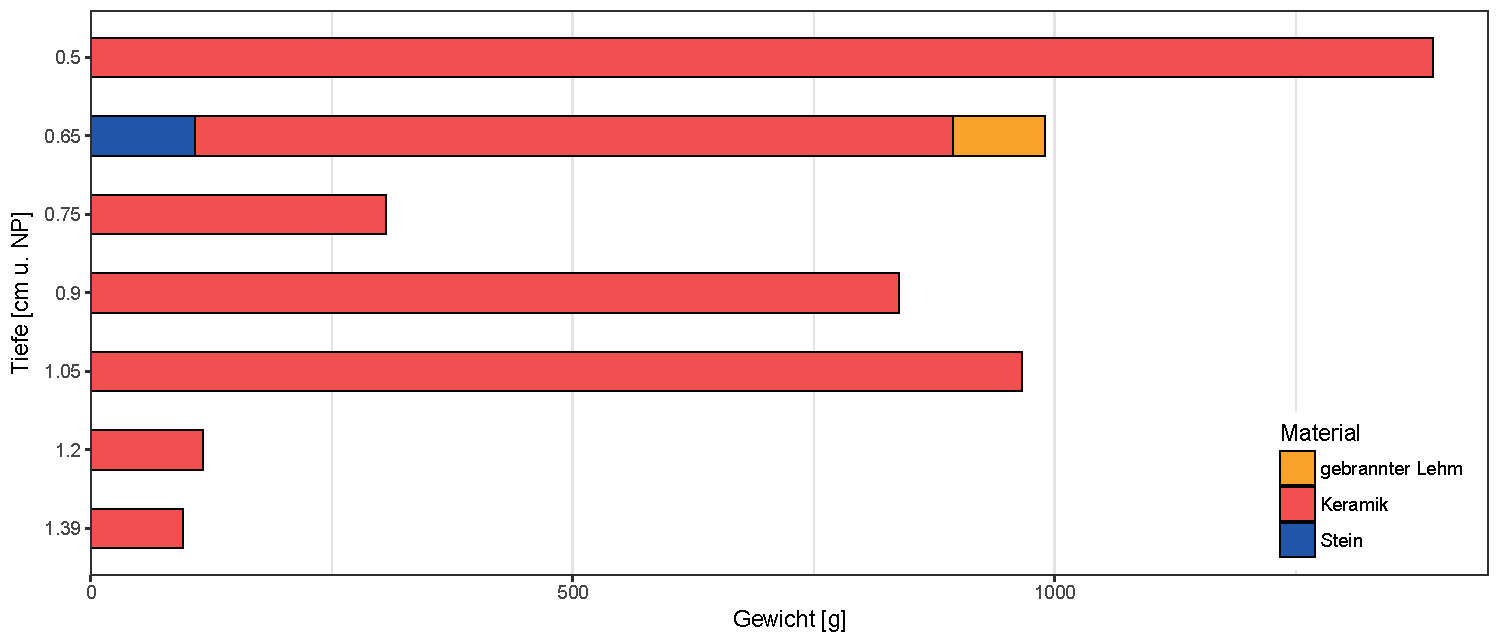
\includegraphics[width=\textwidth]{fig/9-1_MLB85-131_VerteilungFunde_R.pdf}
		\caption{Fundmaterial.\vspace{1em}}
		\label{fig:MLB85-1_VerteilungFunde}
	\end{subfigure}
	\begin{subfigure}[t]{\textwidth}
		\centering
		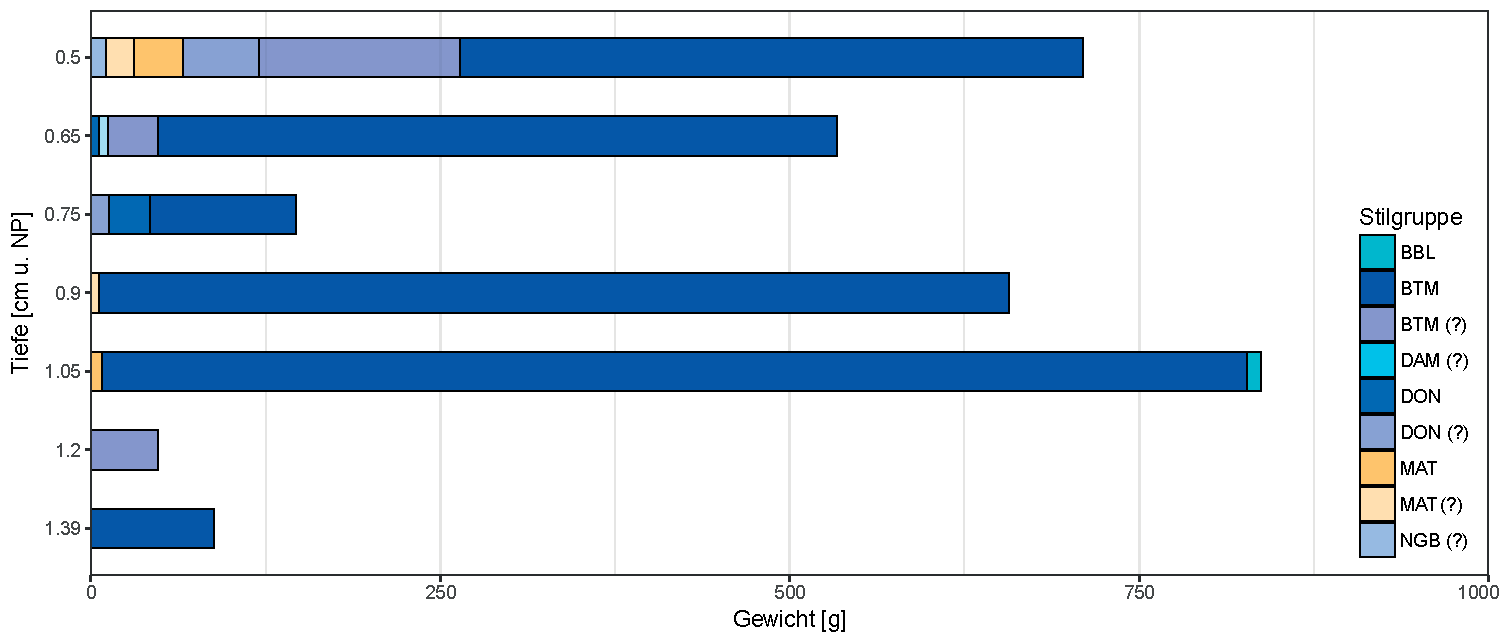
\includegraphics[width=\textwidth]{fig/9-1_MLB85-131_KeramikStilgruppen_R.pdf}
		\caption{Keramische Stilgruppen.\vspace{1em}}
		\label{fig:MLB85-1_KeramikStilgruppen}
	\end{subfigure}
	\begin{subfigure}[t]{\textwidth}
		\centering
		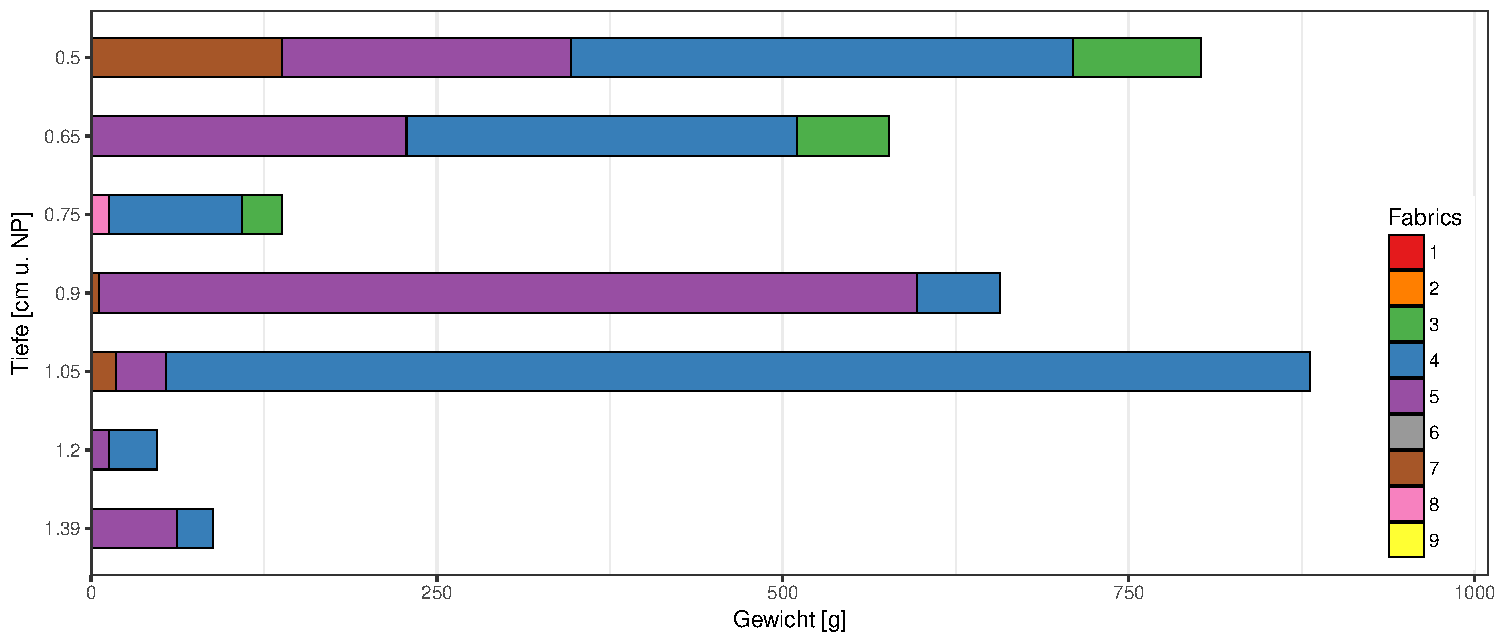
\includegraphics[width=\textwidth]{fig/9-1_MLB85-131_Fabrics_R.pdf}
		\caption{\textit{Fabrics}.}
		\label{fig:MLB85-1_VerteilungFabrics}
	\end{subfigure}
	\caption{MLB 85/1-3-1: Verteilung der Fundmaterialien (A), keramischen Stilgruppen (B) und \textit{Fabrics} (C) in den entsprechenden Tiefen der Grabung.}
	\label{fig:MLB85-1_Verteilung}
\end{figure*}

\vspace{.5em}
\noindent Das Fundmaterial aus der Grube MLB~85/1-3-1 bildet -- zusammen mit jenem aus der benachbarten Grube MLB~85/1-3-2 (Kat.-Nr.~2) -- den Grundstock für den Formenkatalog des Batalimo-Maluba-Stils (Kap.~\ref{sec:BTM-Gr}). Neben der Keramik fand sich ein Stück gebrannten Lehms sowie zwei Steine (Tab.~\ref{tab:MLB85-1-3-1_Funde}). Während der obersten drei Abträge konnten die einzelnen Befunde -- MLB~85/1-3-1, MLB~85/1-3-2 (Kat.-Nr.~2) und MLB~85/1-4-3 (Kat.-Nr.~3) -- nicht unterschieden werden. Die Funde aus diesem Bereich müssen daher als vermischt gelten. Eine Trennung der Funde nach den entsprechenden Komplexen war auch im Rahmen der Auswertung nicht möglich. Das keramische Fundgut ist stark zerscherbt (Abb.~\ref{fig:Fragmenierung_MLB85-131}) und direkte Anpassungen zwischen Scherben ergaben sich äußerst selten (Abb.~\ref{fig:Fragmenierung_MLB85-131}). Dies deutet an, dass es sich bei dem Befund nicht um eine Deponierung von ursprünglich ganzen Gefäßen handelt, sondern dass die Keramik bereits zerscherbt war, als sie in die Grube gelangte. Komplette Gefäße ließen sich kaum rekonstruieren. Die vollständigste Gefäßeinheit (Taf.~25.8) besteht aus 27 Scherben, welche über vier Abträge verteilt sind.\footnote{GE~4 setzt sich aus je zwei Scherben der Abträge 2 und 3 sowie 18 Scherben des 4. und vier weiteren Scherben des 5. Abtrages zusammen.\label{ftn:MLB85-131Refit}}

\begin{table*}[!tb]
	{\footnotesize
		\begin{sftabular}{@{}p{.125\textwidth}p{.125\textwidth}p{.25\textwidth}p{.2\textwidth}p{.15\textwidth}@{}}
			\toprule 
			\textbf{Lab-Nr} & \textbf{Datum (bp)} & \textbf{Datum (2-Sigma)} & \textbf{Abtrag} & \textbf{Tiefe (unter NP)} \\ 
			\midrule 
			GrN-13584 & 1670\( \pm \)110 & 125--605 n.~Chr. & 5 (MLB 85/1-3-1-2; HK 18) & 0,9--1,05\,m \\ 
			KI-2444 & 1930\( \pm \)120 & 342--327 v.~Chr. (0,6\,\%) 204 v.~Chr.--383 n.~Chr. (94,8\,\%) & 7 (MLB 85/1-3-1-4; HK 26) & 1,2--1,39\,m \\ 
			\bottomrule 
	\end{sftabular}}
	\caption{MLB 85/1-3-1: \textsuperscript{14}C-Datierungen.}
	\label{tab:MLB85_1-3-1_14C-Daten}
\end{table*}

\begin{figure*}[!tb]
	\centering
	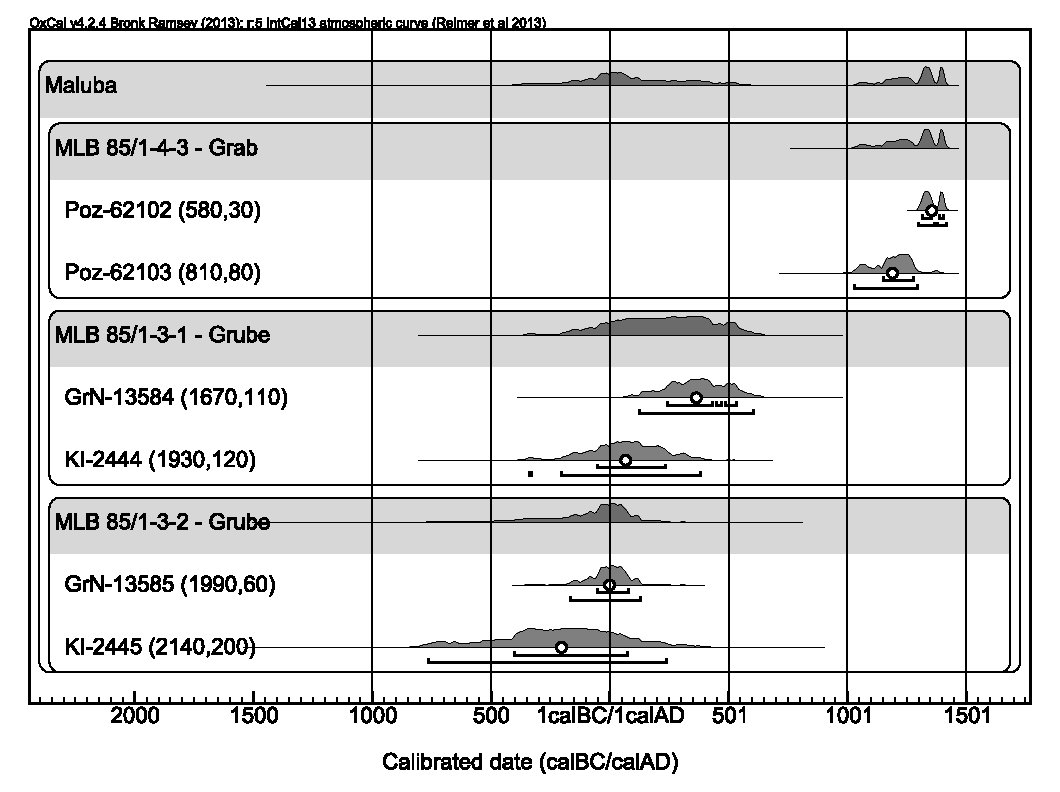
\includegraphics[width = .75\textwidth]{fig/MLB85_14C.pdf}
	\caption{Maluba: Kalibrierung der \textsuperscript{14}C-Datierungen aus den beiden Gruben MLB~85/1-3-1 und MLB~85/1-3-2 sowie der Sekundärbestattung MLB~85/1-4-3 in Maluba am Lua in stratigrafischer Sortierung.}
	\label{fig:MLB85_1_14C-Kalibration}
\end{figure*}

Keramik, insbesondere Vertreter des Batalimo-Maluba-Stils, wurde vor allem in den Abträgen 1--2 und 4--5 gefunden (Abb.~\ref{fig:MLB85-1_Verteilung}). Nach dem fünften Abtrag reduziert sich das Fundaufkommen merklich. Bis in diese Tiefe ist das Inventar mit Scherben durchsetzt, die nicht Teil des Batalimo-Maluba-Stils sind.\footnote{Es handelt sich hierbei um eine GE aus rotbrennenden Tonen mit feiner Matrix (\textit{Fabric} 7) mit sehr kurzen, umgelegten Rändern des Matoto-Stils (Abb.~\ref{fig:MLB85-1_VerteilungFabrics}, Kap.~\ref{sec:MAT-Gr}). In den oberen drei Abträgen fanden sich zudem rouletteverzierte Scherben, von denen eine der Dama-Gruppe zugewiesen werden konnte (Abb.~\ref{fig:MLB85-1_KeramikStilgruppen}; Kap.~\ref{sec:DAM-Gr}).} Diese Verteilung beziehungsweise das auffällig geringe Fundaufkommen im dritten Abtrag kann damit erklärt werden, dass der Abtrag etwas flacher als die anderen war und genau die Grenze zwischen der \textit{Deckschicht} (Abb.~\ref{fig:MLB85_1_Zeichnung}:1) und dem noch erhalten Abschnitt der Grubenverfüllung (2--3) abdeckt. Mit dem vierten Abtrag wurde die Grubenverfüllung ausgegraben, die nunmehr lediglich durch die Sekundärbestattung MLB~85/1-4-3 (Kat.-Nr.~3) gestört war. Der Umstand, dass Anpassungen zwischen Scherben aus dem zweiten bis fünften Abtrag beobachtet wurden\footnote{Siehe Anm.~\ref{ftn:MLB85-131Refit}.}, zeigt an, dass die Abträge 1--3 umgelagertes Grubensediment widerspiegeln. Diese Bereiche sind auch regelhaft mit jüngeren Scherben der Stile Dongo (Kap.~\ref{sec:DON-Gr}), Bobulu (Kap.~\ref{sec:BBL-Gr}), Dama (Kap.~\ref{sec:DAM-Gr}) und Matoto (Kap.~\ref{sec:MAT-Gr}) durchsetzt. Der dritte Abtrag kann als \textit{Störungszone} interpretiert werden. In dieser Tiefe wurde die ursprüngliche Grube mutmaßlich gekappt. Im Profil ist eine deutliche Grenze zwischen den Schichten 1 und 2 (Abb.~\ref{fig:MLB85_1_Zeichnung}) sichtbar. Unterhalb dieser findet sich auffällig viel Holzkohle. 

Das keramische Inventar des Befunds MLB~85/1-3-1 umfasst 99~GE. Aufgrund der starken Fragmentierung ergaben nur zwei GE hinreichend viel Material, um sie als Gefäße anzusprechen. Das Gros bilden 45 Randscherben und 49 Wandungsscherben. Zudem konnten drei Bodenscherben identifiziert werden. Die individuell aufgenommenen GE repräsentieren etwas über 70\,\% des keramischen Materials aus dem Befund.\footnote{Die restlichen, lediglich ausgezählten Scherben sind nicht signifikant oder zeigen nur schlecht ansprechbare Verzierungselemente; beispielsweise einzelne Rillen.}\columnbreak

Der Großteil der identifizierten Gefäßformen sind geschlossene Gefäße mit Zylinderhals und ausbiegendem Rand des Typs C2, wie sie für die Batalimo-Maluba-Gruppe typisch sind (Kap.~\ref{sec:BTM-Gr}). Daneben finden sich nur wenige offene Formen. Es handelt sich hierbei hauptsächlich um Schalen des Typs E5. Von insgesamt 34 Randstücken, die dem Batalimo-Maluba-Stil zugerechnet werden können, sind 19 ausbiegende kurze Ränder des Typs B1.1. Sie zeichnen sich regelhaft durch gerillte Randabschlüsse und Rillenzier auf der Innenseite aus. Für die Matoto-Gruppe charakteristische, kurz umgelegte Ränder des Typs A2 ließen sich in sechs Fällen beobachten. Die entsprechenden Stücke stammen ausschließlich aus dem vierten und fünften Abtrag.\footnote{Diese Stücke, obschon es während der Grabung nicht entsprechend gekennzeichnet wurde, sind mit starker Sicherheit Teil der Verfüllung der jüngeren Bestattung MLB~85/1-4-3 (Kat.-Nr.~3).} Verzierungen basieren größtenteils auf unterschiedlichen Rillen und Riefen-Mustern. Vor allem an der Innenseite der Ränder findet sich regelhaft Rillenverzierung. Die in Batalimo recht häufigen Karo- beziehungsweise Schachbrettmuster (\textsc{De Bayle des Hermens} 1975: Taf.~34) kommen in MLB~85/1-3-1 ebenfalls vor, während Winkelmuster deutlich seltener beobachtet wurden.

\paragraph{Sonstige Funde}\hspace{-.5em}|\hspace{.5em}%
Im zweiten Abtrag fand sich wenig Holzkohle und etwas verziegelter Lehm (Abb.~\ref{fig:MLB85-1_VerteilungFunde}). Ein Stück gebrannter Hüttenlehm weist deutliche konkave Abdrücke auf und kann als Wandbewurf gedeutet werden.\footnote{Siehe auch Diskussion unten im Zusammenhang mit dem in der Grube MLB~85/1-3-2 (Kat.-Nr.~2) gefundenen Hüttenlehm.} Zudem wurden zwei kleine Sandsteinfragmente ausgegraben, die zusammen nur etwa 100\,g wiegen und keine Bearbeitungsspuren zeigen.

\begin{figure*}[!tb]
	\begin{subfigure}{0.37\textwidth}
		\centering
		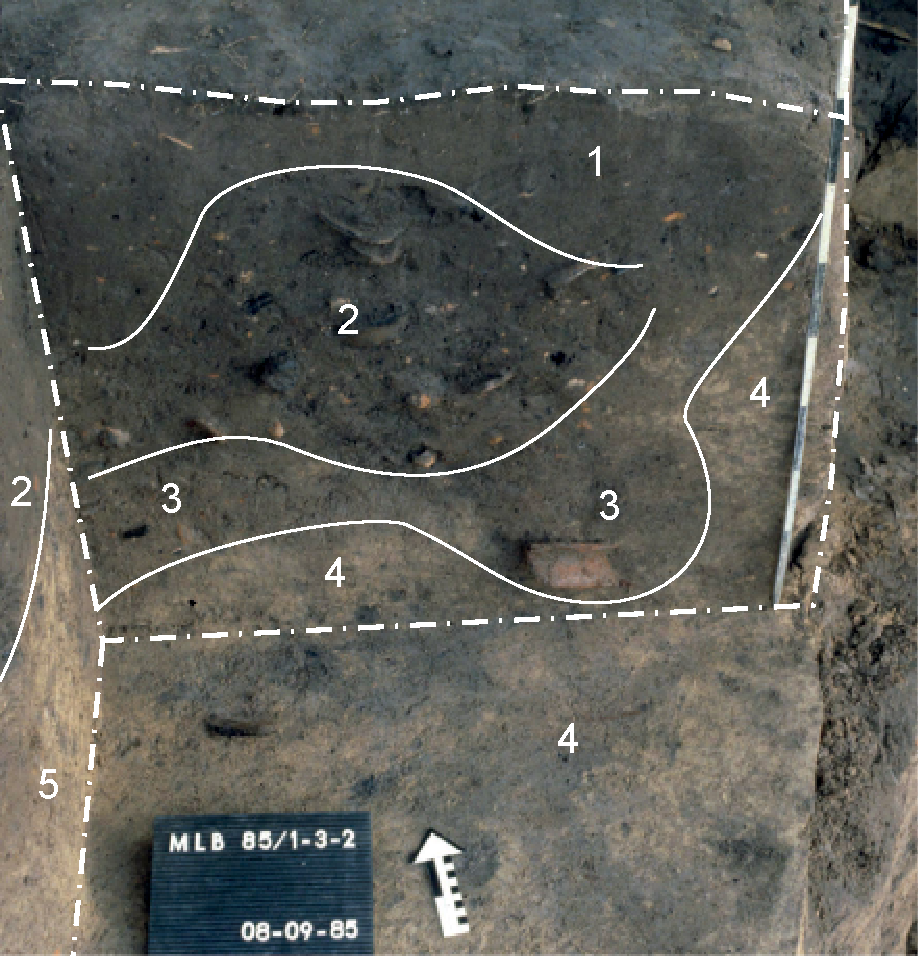
\includegraphics[width=\textwidth]{fig/MLB85-132_E85-032-23.pdf}
		\caption{West--Ost-Profil}
		\label{fig:MLB85-132_W-O-Prof}
	\end{subfigure}\hspace{0.01\textwidth}
	\begin{subfigure}{0.61\textwidth}
		\centering
		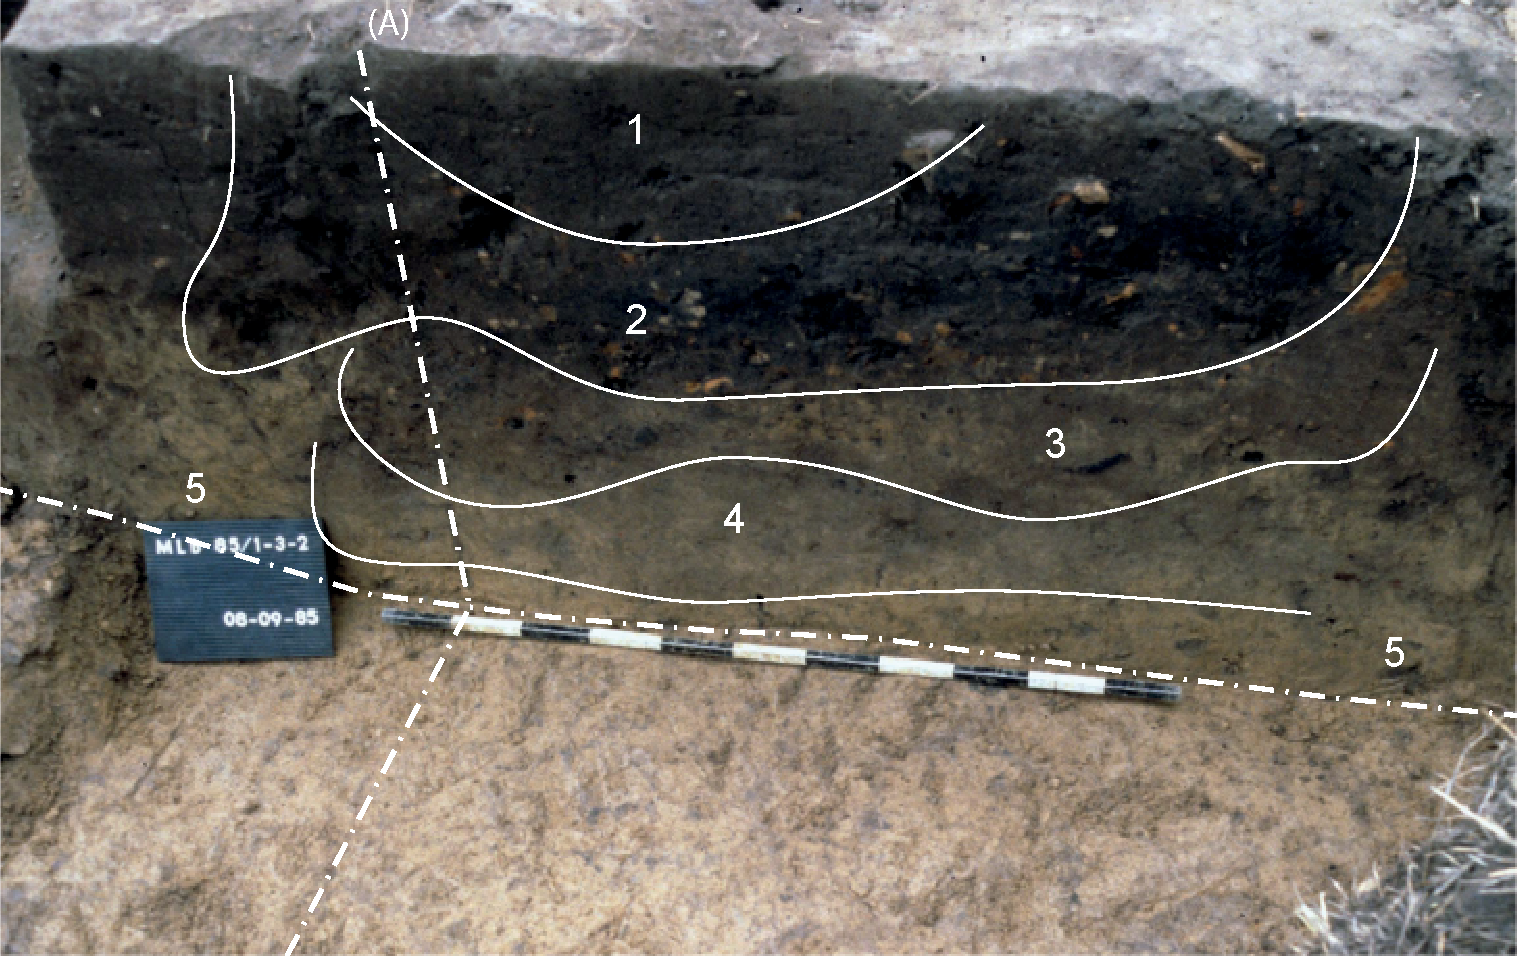
\includegraphics[width=\textwidth]{fig/MLB85-132_E85-032-27.pdf}
		\caption{Nord--Süd-Profil}
		\label{fig:MLB85-132_N-S-Prof}
	\end{subfigure}
	\caption{MLB~85/1-3-2: West--Ost-orientiertes Profil (A) und Süd--Nord-orientiertes Profil durch den Befund bei Grabungsabschluss (B). Zur Lage der Profile siehe auch Abb.~\ref{fig:MLB85_1_Zeichnung} (Fotos: M. K. H. Eggert, 1985).}
	\label{fig:MLB85-1-3-2_NordProfil}
\end{figure*}

\paragraph{Datierung}\hspace{-.5em}|\hspace{.5em}%
Je eine Probe für Radiokohlenstoffdatierungen wurde im fünften wie siebten Abtrag genommen (Tab.~\ref{tab:MLB85_1-3-1_14C-Daten}). Beide absolute Datierungen decken einen Bereich zwischen dem 4.~Jh. v.~Chr. bis 6.~Jh. n.~Chr. ab. Während die Probe aus dem fünften Abtrag (GrN-13584) etwas jünger als die aus dem siebten Abtrag stammende Probe (KI-2444) datiert, überlagern sich beide Proben im kalbierten 2-Sigma-Intervall. Für den Befund MLB~85/1-3-1 lässt sich eine Datierung in die erste Hälfte des 1.~Jt. n.~Chr. als am Wahrscheinlichsten annehmen (Abb.~\ref{fig:MLB85_1_14C-Kalibration}). 

\paragraph{Interpretation}\hspace{-.5em}|\hspace{.5em}%
Die in der Grabung MLB~85/1-3-1 erfasste Grube weist einen Durchmesser von zirka 1,5\,m auf und reicht noch bis zu 1,1\,m unter die rezente Oberfläche. Zum Zeitpunkt der Grabung waren bereits etwa 40\,\% des Befundes erodiert. Die gesamte Grube, vorausgesetzt sie war zylindrisch, müsste in etwa ein Volumen von etwa 1,4\,m\textsuperscript{3} aufgewiesen haben, von denen noch etwa 0,9\,m\textsuperscript{3} erhalten waren. Die Funddichte liegt bei etwa 5\,kg/m\textsuperscript{3} und das Fundaufkommen nimmt zur Sohle hin deutlich ab. Ausreichend gesichert ist die Verfüllung der Grube erst ab einer Tiefe von etwa 0,3\,m unter der rezenten Oberfläche. Ob die Durchmischung im darüber liegenden Bereich das Ergebnis jüngerer Eingrabungen ist, konnte nicht abschließend geklärt werden. Das keramische Fundmaterial aus der Grube ist einer der definierenden Komplexe für die Beschreibung des Batalimo-Maluba-Stils. Die Auswertung ergab keine Hinweise, welche Rückschlüsse auf die Nutzung oder Funktion der Grube zuließen. Charakteristika einer intentionellen Deponierung \parencite[siehe][]{Wotzka.1993} fanden sich nicht.